% file thesis.tex
% Archivo thesis.tex
% Documento maestro que incluye todos los paquetes necesarios para el documento
% principal.

% Documento obtenido por un sinfin de iteraciones de administradores del LDC
% Estructura actual hecha por:
% Jairo Lopez <jairo@ldc.usb.ve>
% Actualizado ligeramente por:
% Alexander Tough 

\documentclass[oneside,12pt,letterpaper]{report}
\tolerance=1000  
\hbadness=10000  
\raggedbottom

% Paquetes para manejar graficos
\usepackage{epsf}
\usepackage[pdftex]{graphicx}
\usepackage{epsfig}
% Simbolos matematicos
\usepackage{latexsym,amssymb}
% Paquetes para presentar una tesis decente.
\usepackage{setspace,cite} % Doble espacio para texto, espacio singular para
                           % los caption y pie de pagina

% Paquetes no utilizados para citas
%\usepackage{mcite} 
%\usepackage{draft} 

\usepackage{wrapfig}
\usepackage{alltt}

% Acentos 
\usepackage[spanish,activeacute]{babel}
\usepackage[spanish]{translator}
\usepackage[utf8]{inputenc}
\usepackage{color, xcolor, colortbl}
\usepackage{multirow}
\usepackage{subfig}
\usepackage[OT1]{fontenc}
\usepackage{tocbibind}
\usepackage{anysize}
\usepackage{listings} 

% Para poder tener texto asiatico
%\usepackage{CJK}

% Opciones para los glosarios
\usepackage[style=altlist,toc,numberline,acronym]{glossaries}
\usepackage{url}
\usepackage{amsthm}
\usepackage{amsmath}
\usepackage{fancyhdr} % Necesario para los encabezados
\usepackage{fancyvrb}
\usepackage{makeidx} % En caso de necesitar indices.
\makeindex  % Necesitado para los indices

% Definiciones para definicions, teoremas y lemas
\theoremstyle{definition} \newtheorem{definicion}{Definici\'{o}n}
\theoremstyle{plain} \newtheorem{teorema}{Teorema}
\theoremstyle{plain} \newtheorem{lema}{Lema}

% Para la creacion de los pdfs
\usepackage{hyperref}

% Para resolver el lio del Unicode para la informacion de los PDFs
% En pdftitle coloca el nombre de su proyecto de grado/pasantia.
% En pdfauthor coloca su nombre.
\hypersetup{
    pdftitle = {TITULO DEL PROYECTO DE GRADO},
    pdfauthor={AUTOR},
    colorlinks,
    citecolor=black,
    filecolor=black,
    linkcolor=black,
    urlcolor=black,
    backref,
    pdftex
}

% Crea el glosario
\makeglossaries

% Incluye el glosario
\newacronym{as-h}{as-H}{proceso autosimilar con par\'{a}metro autosimilar $H$}

\newacronym{asie-h}{asie-H}{proceso autosimilar con par\'{a}metro autosimilar
$H$ e incrementos estacionarios}

\newacronym{aas-h}{aas-H}{proceso asint\'{o}ticamente autosimilar con
par\'{a}metro autosimilar $H$}


% Para crear la hoja escaneada de las firmas
\usepackage[absolute]{textpos}

% Pone los nombres y las opciones para mostrar los codigos fuentes
\lstset{language=C, breaklines=true, frame=single, showstringspaces=false,
        showtabs=false, numbers=left, keywordstyle=\color{black},
        basicstyle=\footnotesize, captionpos=b }
\renewcommand{\lstlistingname}{C\'{o}digo fuente}
\renewcommand{\lstlistlistingname}{\'{I}ndice de c\'{o}digos fuentes}

% Dimensiones de la pagina
\setlength{\headheight}{15pt}
\marginsize{3cm}{2cm}{2cm}{2cm}

% Se pueden omitir para que no compile ciertos capitulos.
\includeonly{header, intro, ssimilar, herramienta, resultados, conclusiones}

%%%%%%%%%%%%%%%%%%%%%%%%%%%%%%%%%%%%%%%%%%%%%%%%%%%%%%%%%%%%%%%%%%%%%%%%%%%
%%%%%%%%%%%%%%%%      end of preamble and start of document     %%%%%%%%%%%
%%%%%%%%%%%%%%%%%%%%%%%%%%%%%%%%%%%%%%%%%%%%%%%%%%%%%%%%%%%%%%%%%%%%%%%%%%%
\begin{document}

% Pagina de titulo
% Pagina de titulo
\begin{titlepage}
\begin{center}

% Upper part (aqui ya esta incluido el logo de la USB).

\includegraphics[scale=0.5,type=png,ext=.png,read=.png]{figures/cebolla} \\

% Encabezado
\textsc {\large UNIVERSIDAD SIM'ON BOL'IVAR} \\
\textsc{\bfseries DECANATO DE ESTUDIOS PROFESIONALES\\
COORDINACI'ON DE INGENIER'IA DE LA COMPUTACI'ON}

\bigskip
\bigskip
\bigskip
\bigskip
\bigskip
\bigskip
\bigskip
\bigskip
\bigskip

% Title/Titulo
% Aqui ponga el nombre de su proyecto de grado/pasantia larga
\textsc{\bfseries Clustering de datos numericos por medio de algoritmos basados en poblacion e inteligencia colectiva}

\bigskip
\bigskip
\bigskip
\bigskip
\bigskip

% Author and supervisor/Autor y tutor
\begin{minipage}{\textwidth}
\centering
Por: \\
Alexander De Sousa\\
Federico Ponte \\

\bigskip
\bigskip
\bigskip

Realizado con la asesor'ia de: \\
Emely Arra\'iz
\end{minipage}

\bigskip
\bigskip
\bigskip
\bigskip
\bigskip
\bigskip
\bigskip
\bigskip
\bigskip

% Bottom half
{PROYECTO DE GRADO \\ Presentado ante la Ilustre Universidad Sim'on Bol'ivar \\
como requisito parcial para optar al t'itulo de \\ Ingeniero en Computaci'on} \\

\bigskip
\bigskip
\vfill

% Date/Fecha 
{\large \bfseries Sartenejas, FECHA (MES de A\~NO)}

\end{center}
\end{titlepage}


% Pagina de acta final (vacio)
% Pagina del acta final
\begin{titlepage}
\begin{center}

% Upper part

\includegraphics[scale=0.5,type=png,ext=.png,read=.png]{figures/cebolla} \\

\textsc {\large UNIVERSIDAD SIM'ON BOL'IVAR} \\
\textsc{DECANATO DE ESTUDIOS PROFESIONALES\\
COORDINACI'ON DE INGENIER'IA DE LA COMPUTACI'ON}

\bigskip
\bigskip
\bigskip
\bigskip
\bigskip
\bigskip

% Title
\textsc{ACTA FINAL PROYECTO DE GRADO}

\bigskip
\bigskip

% Aqui coloca el nombre de su proyecto de grado/pasantia larga.
\textsc{\bfseries Clustering de datos numericos por medio de algoritmos basados en poblacion e inteligencia colectiva}

\bigskip
\bigskip
\bigskip
\bigskip

\begin{minipage}{\textwidth}
\centering
Presentado por: \\
% Aqui coloca su nombre.
\textsc{\bfseries Alexander De Sousa} \\
\textsc{\bfseries Federico Ponte} \\

\bigskip
\bigskip
\bigskip
\bigskip

Este Proyecto de Grado ha sido aprobado por el siguiente jurado examinador: \\

\bigskip
\bigskip

% Despues de cada line coloca el (los) nombre(s) de
% cada uno de los integrantes del jurado.
\line(1,0){200} \\
PROFESOR 1\\

\bigskip
\bigskip

\line(1,0){200} \\
PROFESOR 2 \\

\bigskip
\bigskip

\line(1,0){200} \\
PROFESOR 3 \\
\end{minipage}

\bigskip
\bigskip
\vfill

% Date/Fecha
{\large \bfseries Sartenejas, FECHA (dd/mm/aa)}

\end{center}
\end{titlepage}


\setcounter{secnumdepth}{3}
\setcounter{tocdepth}{4}

% Define encabezado numeros romanos y como se separan los captiulos y las
% secciones
\addtolength{\headheight}{3pt}
\pagenumbering{roman}
\pagestyle{fancyplain}

\renewcommand{\chaptermark}[1]{\markboth{\chaptername\ \thechapter:\,\ #1}{}}
\renewcommand{\sectionmark}[1]{\markright{\thesection\,\ #1}}

\onehalfspacing

\lhead{}
\chead{}
\rhead{}
\renewcommand{\headrulewidth}{0.0pt}
\lfoot{}
\cfoot{\fancyplain{}{\thepage}}
\rfoot{}


% Pagina de resumen
\vspace{5 mm}

\setcounter{page}{4}
\begin{center}
	{\bf Resumen}
\end{center}

\vspace{5 mm}

La agrupación de datos (\emph{data clustering}) es el proceso de particionar una
colección de datos en conjuntos de clases significativas, llamadas \emph{clusters},
donde los objetos de una clase comparten ca\-rac\-te\-rís\-ti\-cas comunes. En este trabajo,
se presenta un estudio comparativo de cinco metaheurísticas basadas en población
e inteligencia colectiva (\emph{algoritmo genético}, \emph{optimizador de enjambre
de partículas}, \emph{evolución diferencial}, \emph{algoritmo de abeja} y
\emph{algoritmo de clustering de hormigas}) para resolver el problema de \emph{data
clustering} en calidad de soluciones finales. Los datos usados para el estudio son
de tipo numérico, comúnmente utilizados en la literatura afín. Del estudio se
llega a la conclusión que para resolver el problema de \emph{clustering} de datos
numéricos se deben utilizar el \emph{algoritmo genético} o el \emph{algoritmo de
abeja}, ambos hibridados con la heurística \emph{K-means} como método de mejoramiento
de las soluciones finales.

\newpage



% Pagina de dedicatoria (opcional)
\setcounter{page}{5}

\vspace*{8cm} 
\pdfbookmark[0]{Dedication}{dedication} % Sets a PDF bookmark for the dedication
\begin{center} 
\large DEDICATORIA
\end{center}
\newpage


% Pagina de agradecimientos (opcional)
\setcounter{page}{6}

\chapter*{Agradecimientos
\markboth{Agradecimientos}{Agradecimientos}}
A todas las personas que aportaron su granito de arena en la realización de este
proyecto de grado, en especial, nuestra tutora.


% Crea la tabla de contenidos
\tableofcontents

% Crea la lista de cuadros
\listoftables

% Crea la lista de figuras
\listoffigures

% Crea la lista de codigos fuentes
%\lstlistoflistings

\clearpage

% Define encabezado en numeros arabicos  
\pagenumbering{arabic}

\fancyhf{} % Redefine el encabezado 
\lhead{}
\chead{}
\rhead{\fancyplain{}{\thepage}}
\renewcommand{\headrulewidth}{0.0pt}
\lfoot{}
\cfoot{}
\rfoot{}

\doublespacing


% Incluye los archivos deseados - El contenido de
% su proyecto de grado/pasantia larga.
 \addcontentsline{toc}{chapter}{Introducci\'on}

% Titulo de la introduccion.
\begin{center}
	{\bf Introducci\'on} \label{chap:intro}
\end{center}

% Contenido de la introduccion.

\label{sect:motivacion}
%Puedes quitar esto(es opcional)
\vspace{5 mm}

En la Universidad Sim\'on Bol\'ivar es dictada la materia electiva
Dise\~no de Algoritmos II, en la cual se enseñan diversas metaheur\'isticas.
El curso es dividido en grupos (normalmente en parejas) y a cada uno se le asigna un problema 
de optimizaci\'on NP-hard para resolver mediante estos m\'etodos. Uno de \'estos es Data Clustering.
Consiste m\'etodo de crear grupos de objetos,
de tal manera que los objetos dentro de un cluster sean similares y 
en clusters distintos sean diferentes. \cite{GaChJi2007}

%Puedes quitar esto(es opcional)
\vspace{5 mm}

\label{sect:justificacion}
%Puedes quitar esto(es opcional)
\vspace{5 mm}

Se sabe que hoy en d\'ia hay muchos avances y usos del reconocimiento de im\'agenes.
Ejemplos son Google Goggles, diversos m\'odulos de JDownloader con el objetivo de reconocer
captchas, reconocimiento de caras por parte de las c\'amaras, etc. Un algoritmo de
Data Clustering sirve como entrada para un modelo basado en sistemas de
reconocimiento de objetos. Tambi\'en el poder encontrar patrones escondido en
conjuntos de datos es muy \'util: una empresa podr\'ia mejorar su ventas.

%Puedes quitar esto(es opcional)
\vspace{5 mm}

\label{sect:planteamiento}
%Puedes quitar esto(es opcional)
\vspace{5 mm}

Actualmente existe una ardua investigaci\'on en diversas metaheur\'isticas para
resolver diversos problemas optimizaci\'on. La idea es obtener en un tiempo
considerable una respuesta \'optima o lo m\'as cercano posible a \'esta. Por
ello muchos cient\'ificos han empezado a inspirarse en la naturaleza.
Una profunda obsevaci\'on en la relaci\'on subyacente 
entre \'esta y optimizaci\'on ha llevado al desarrollo de nuevos paradigmas
para lograr este objetivo\cite{SwAjAm2009}. De ac\'a surgen las basadas en poblaci\'on e inteligencia
colectiva.

Los m\'as prominentes y prometedores son el algoritmo g\'enetico, abeja, DE, hormiga
y PSO. Todos constan de un grupo de individuos que van a ir modificandose a trav\'es
del tiempo. La forma en que se den estos cambios depende de cada algoritmo.

%Puedes quitar esto(es opcional)
\vspace{5 mm}

\label{sect:objetivo_general}
%Puedes quitar esto(es opcional)
\vspace{5 mm}

El objetivo principal es la implementaci\'on de \'estas cinco metaheur\'isticas
y el K-means, el algoritmo m\'as famoso para data clustering, para ver la calidad
de cada uno y compararlos entre si. \'Esta debe ser eficiente, rapida y flexible
con el objetivo de que pueda ser usada a futuro por otras personas y lograr
comprar los algoritmos de la forma m\'as efectiva.


%Puedes quitar esto(es opcional)
\vspace{5 mm}

\label{sect:objetivos_especificos}
%Puedes quitar esto(es opcional)
\vspace{5 mm}

El programa debe tener la capcidad de leer archivos en formato CSV e im\'agenes
en formato PNG y TIFF (las im\'agenes son datos n\'umericos). La salida tiene que ser
concorde al tipo de cada archivo, para un csv un archivo de texto y
en el otro caso una imagen con un color para cada grupo creado. Es necesario que
el lenguaje que se use tenga la capcidad de compilar a c\'odigo de m\'aquina
en vista que se busca eficiencia en tiempo.

Para comparar las diversas metaheur\'sticas es esencial tener una m\'etrica com\'un
con ese fin. Adem\'as se debe colocar un limite de tiempo en las corridas para 
obtener una buena soluci\'on en un tiempo considerable.



% Marco Teorico.
\chapter{Marco te'orico} \label{chap:ssimilar}

\vspace{5 mm}

\section{Data Clustering} \label{sect:dclust}

\subsection{Introducci\'on} \label{sect:dclusti}

Data clustering (o s\'olo clustering), tambien llamado an\'alisis de clusters, an\'alisis de segmentaci\'on,
an\'alisis de taxionom\'ia, o clasificaci\'on no supervisada, es un m\'etodo de crear grupos de objetos,
o clusters, de tal manera que cada los objetos dentro de un cluster sean similares y los objetos 
en clusters distintos sean diferents. \cite{GaChJi2007}

En \cite{SwAjAm2009} hablan de ciertos puntos importantes:

\begin{itemize}

\item Hay muchas definciones porpuestas por una diversa cantidad de personas,
 lo que demuestra la dificultad de proveer una \'unica definici\'on formal. Ésto radica en que
es bastante complejo capturar por los medios de cualquier criterio individual que se 
use la noci\'on que tiene un humano. El siguiente ejemplo va a poner en claro.

Considere los siguientes animales: oveja, perro, gato (mam\'iferos), gorri\'on, gaviota (aves),
v\'ivora, lagarto (rept\'iles), pez de colores, salmonete, tibur\'on azul (peces), y rana (anf\'ibio).
Para organizar estos animales en clusters, se tiene que definir un criterio. Por ello, si 
empleamos la manera en que estos animales llevan a cabo su descendencia, la oveja, perro, gato
y tibur\'on azul van a ser asignados al mismo cluster, mientras que el resto van a dormar un segundo
(Figura \ref{fig:ejemplo1}).  En cambio, si el criterio es la existencia de pulmones, 
el pez de colores, el salmonete y el tibur\'on son
asignados al mismo cluster, mientras que el resto a otro (Figura \ref{fig:ejemplo2}).
 Por otro lado, si el criterio es el ambiente
donde viven los anoamles, la oveja, perro, gato, gorri\'on, gaviota, v\'ivora y el lagarto van a formar un cluster
(viven fuera del agua), el pez de colores, salmonete y el tibur\'on azul van a formar un otro (viven afuera
del agua), y un tercero que va a contener a la rana, ya que puede vivir en los dos (Figura \ref{fig:ejemplo3}). 

\begin{figure}[htb]
\centering
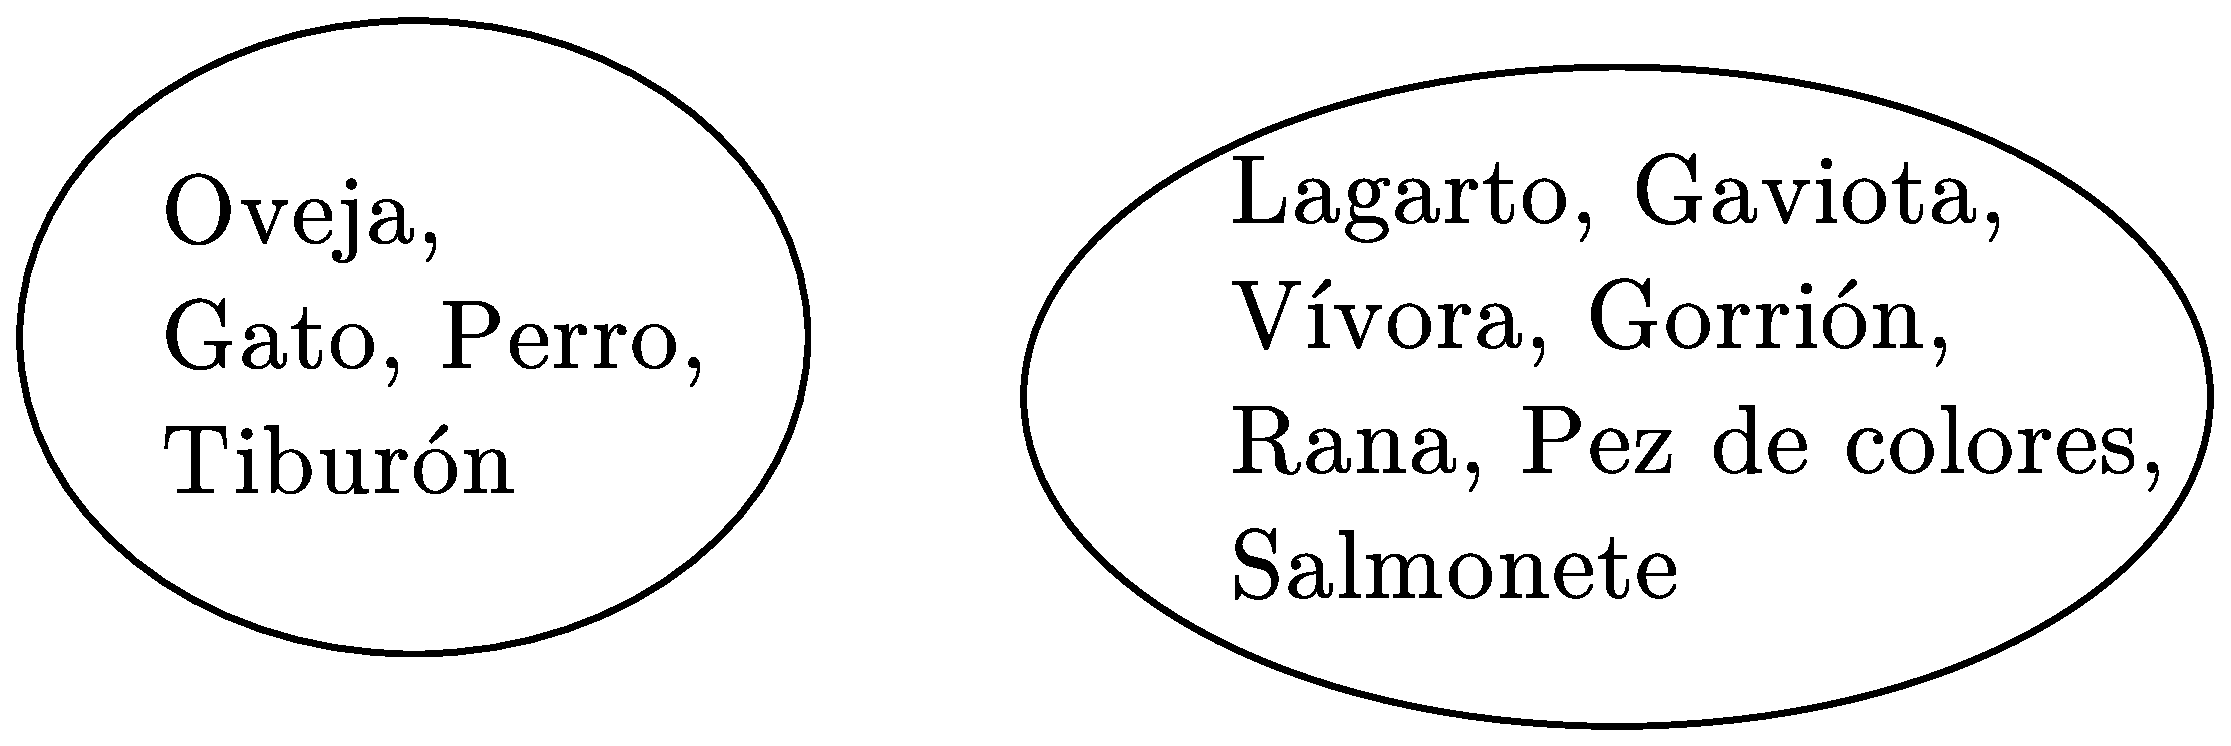
\includegraphics[scale=0.35,type=png,ext=.png,read=.png]{figures/ejemplo1}
\caption{Clustering usando como criterio la manera que llevan a cabo su descendencia}
\label{fig:ejemplo1}
\end{figure}

\begin{figure}[htb]
\centering
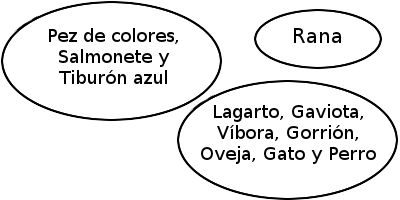
\includegraphics[scale=0.35,type=png,ext=.png,read=.png]{figures/ejemplo2}
\caption{Clustering usando como criterio la existencia de pulmones}
\label{fig:ejemplo2}
\end{figure}

\begin{figure}[htb]
\centering
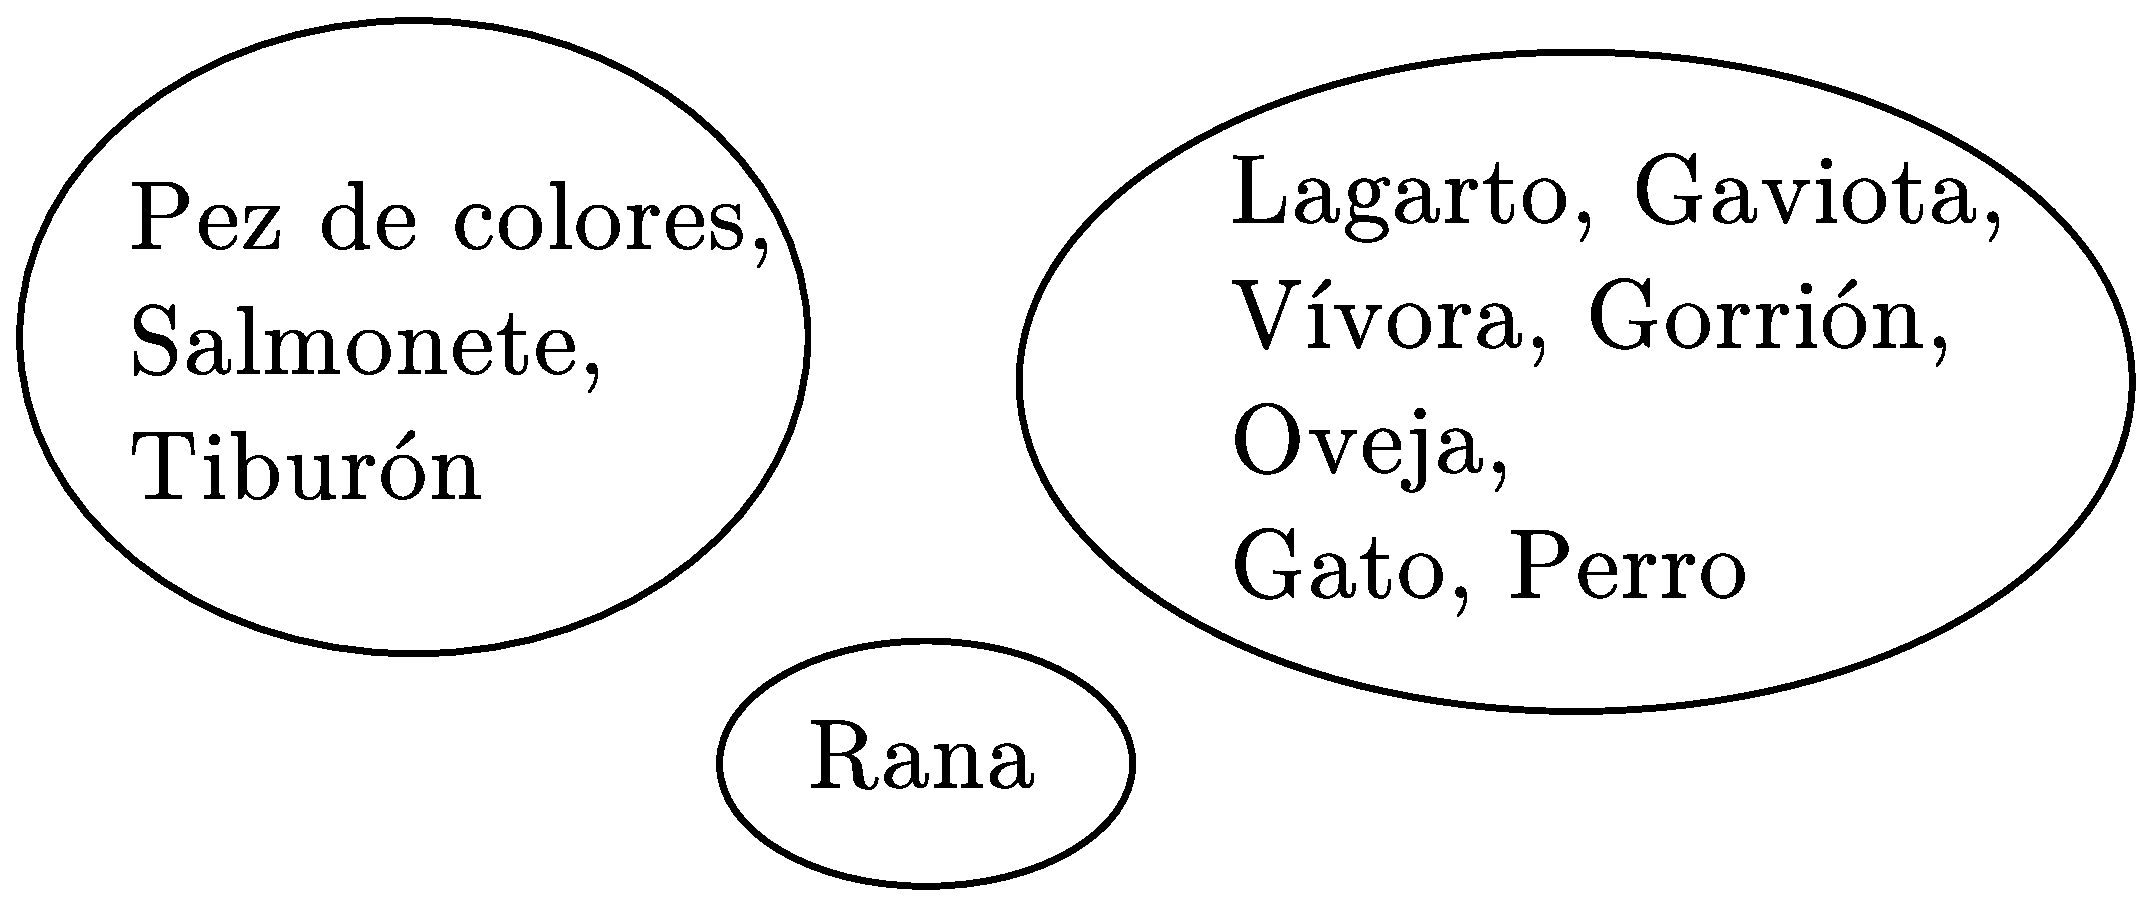
\includegraphics[scale=0.35,type=png,ext=.png,read=.png]{figures/ejemplo3}
\caption{Clustering usado como criterio el ambiente donde viven}
\label{fig:ejemplo3}
\end{figure}

Se puede ver que gracias a la falta de un criterio universal para el clustering,
 \'esta es muy subjetiva en muchos casos.

\item Se puede ver desde el punto de vista de aprendizaje autom\'atico, donde los clusters
correponden a patrones escondidos en los datos, la b\'usqueda de clusters 
es una especie de aprendizaje no supervisado, y el sistema resultante representa
un concepto de datos. Es importante entender la diferencia
entre clustering (aprendizaje no supervisado) y clasificaci\'on supervisada 
(an\'alisis discriminante). En esta \'ultima, se provee una colecci\'on patrones etiquetados
(preclasificados); el problema es etiquetar a un patr\'on recien encontrado, a\'un no etiquetado. 
Tipicamente, los patrones etiquetados (entrenamiento) ya dados son usados para obtener
la descripciones de las clases, que a su vez se utilizan para etiquetar un nuevo patr\'on.
En este caso de clustering, el problema consiste en agrupar una colecci\'on de patrones no etiquetados
en clusters significativos. En este sentidos, las etiquetas se asocian con los clusters tambi\'en,
pero esta categor\'ia de etiquetas son basados en datos, es decir, que se obtienen unicamente
de \'estos.

\item Un algoritmos de clustering se espera que descubra el agrupamiento natural
(pertinente a la noci\'on de los humanos clustering) que existe en una conjunto 
de patrones o puntos de datos. Cada patr\'on puede ser identificado como un punto en un hiperespacio,
llamado espacio de caracter\'isticas, abarcado por las caracter\'isticas asociadas a \'el. La entrada
es un conjunto esos puntos en el espacio carater\'istico multidimensional. Un algoritmo ideal de 
clustering preciso debe presentar como su salida, la etiqueda para cada patr\'on, es decir,
el cluster a cual pertenece cada punto.

\end{itemize}

\'Este problema a sido abordado por diversos campos del conocimiento como la estad\'istica
(an\'aslisis multivariado), teor\'ia de grafos, computaci\'on evolutiva, redes neurales y
as\'i sucesivamente\cite{SwAjAm2009}. Entre sus aplicaciones se encuentra la miner\'ia de datos, expresi\'on de los genes, 
segmentaciones de clientes y procesamiento de im\'agenes, muchas otras. \cite{GaChJi2007}

En especial llama la atenci\'on el \'ultimo mencionado. El procesamiento de im\'agenes es fundamental para los
humanos. Su importancia radica en que la salida puede ser usada como la entrada para 
un modelo basado en sistemas de reconocimiento de objetos.
\'Esto le da una gama de aplicaciones gigantescas: cualquier tipo de reconicimiento de im\'agenes.
Tambi\'en en el \'area m\'edica puede ayudar a encontrar regiones en las im\'agenes que sean tumores,
que posiblemente humano no logre identificar, lo que es extremadamente
\'util.

Brucker en \cite{Br1978} ilustr\'o que el problema es NP-hard cuando el n\'umero 
de clusters excede 3.

\subsection{Definici\'on} \label{sect:dclustdef}

Siguiendo con \cite{SwAjAm2009} antes de dar un definici\'on matem\'atica al problema hay que hablar de 
los siguientes t\'erminos que van a ser usados a trav\'es de la tesis:

\begin{itemize}

\item {\bf Patr\'on o vector caracter\'istico:} Se va a encargar de abstraer matem\'aticamente las
caracter\'isticas que poseen los objetos a los cuales se les har\'a el clustering.

\item {\bf Caracter\'istica:} Es una componente de un patr\'on. \'Esta representa
la base usada para clasificaci\'on de los patrones.

\item {\bf Cluster:} Es un grupo de patrones similares, y los patrones de dos clusters 
distintos no deben ser similares.

\item {\bf Hard clustering:} Cada patr\'on se asigna solamente a un cluster.

\item {\bf Medici\'on de distancia:} Es la m\'etrica con la cual se va a evaluar
la disimilaridad entre los patrones. M\'as adelante se habl\'a en m\'as detalle.

\end{itemize}

Ahora se puede dar una definici\'on formal al problema:

Sea $P = \{ P_1, P_2, \dots , P_N\}$ un conjunto de N patrones, 
donde cada uno tiene M caracter\'isticas. Éstos pueden
ser reprentados por una matriz $Z_{NxM}$. El vector de la fila $i$ caracteriza al 
patr\'on $i$ del conjunto $P$ y cada elemento $Z_{i,j}$ en $Z_i$ su caracter\'istica $j$.
Dada tal matriz Z$_{NxM}$ la idea es que un algoritmo de clustering intente hallar
el particionamiento $C = \{ C_1, C_2, \dots , C_K \}$ tal que los patrones
en el mismo cluster $C_i$ su similaridad sea la mayor y entre clusteres diferentes
sean lo más disimilar:

\begin{enumerate}

\item Cada cluster debe tener por lo menos un patr\'on asignado:

$\forall i | i \in \{1, 2, \dots, K\} : C_i \neq \emptyset$

\item Dos patrones distintos no tienen ning\'un patr\'on en com\'un:

$\forall i,j | i,j\in \{1, 2, \dots, K\} \land i \neq j:  C_i \cap C_j \neq \emptyset$

\item Cada patr\'on debe estar asignado a un cluster:

$\bigcup_{i=1}^{K} C_i = P$

\end{enumerate}

Dado que el conjunto de datos dados puede ser partidionado de varias maneras
manteniendo las propiedades de arriba, es necesaria una función objetico o en otras palabras
una medida de que tan buena es la partici\'on. El problema se comvierte en hallar
una partici\'on $C^*$  \'optima o lo m\'as cercano a ella en comparaci\'on a 
las otras soluciones posible $C = \{ C^1, C^2, \dots, C^{T(N,K)} \}$ donde 
$T(N,K) = { {1 \over K!} \times {\sum_{i=1}^{K} (-1)^i  \binom{K}{i} (K-i)^i} }$
es el n\'umero de particiones posibles. \'Esto es lo mismo que optimizar $f(Z_{NxM}, PC)$,
donde PC es un partici\'on del conjunto C y $f$ es una funci\'on objetivo que
cuantifica la calidad del particionamiento en base a la similaridad o disimilaridad
de los patrones.

\section{Metaheur\'isticas}

\subsection{Abeja}

\subsection{DE}

Es un algoritmo basado en poblaci\'on de
optimizaci\'on global que hace uso de una representaci\'on de punto flotante
(codificaci\'on real), bastante parecido al gen\'etico. Se tienen los pasos de cruce 
y selecci\'on, pero no mutaci\'on.
El $i$-\'esimo vector individual (cromosoma)
de la poblaci\'on con tiempo (generaci\'on) $t$ tiene $d$ componentes
dimensiones:

%Ejemplo de vector.
%INICIO
\begin{center}
$ \overrightarrow{Z_i}(t) = [ Z_{i,1}(t), Z_{i,2}, \cdots, Z_{i,d}(t) ] $
\end{center}
%END

Para cada vector individual $\overrightarrow{Z_k}(t)$ que pertenece
a la poblaci\'on actual, el DE aleatoriamente toma tres individuos
$\overrightarrow{Z_i}(t)$, $\overrightarrow{Z_j}(t)$ y $\overrightarrow{Z_m}(t)$ de la misma generaci\'on (de modo que sean distintos $k$, 
$i$, $j$ y $m$). Entonces calcula la diferencia entre $\overrightarrow{Z_i}(t)$ y $\overrightarrow{Z_j}(t)$, lo escala por un escalar $F$
(usualmente $F \in [0, 1]$) y crea un hijo prueba $\overrightarrow{U_i}(t + 1)$ a\~nadiendo el resultado a $\overrightarrow{Z_m}(t)$. De modo
que para la $n$-\'esima componente del vector:

\[
  U_{k,n}(t+1) =
  \begin{cases}
    Z_{m,n}(t) + F(Z_{i,n}(t) - Z_{j,n}(t))  & \text{si } rand_n(0,1) < Cr\\
    Z_{k,n}(t)                               & \text{sino}
  \end{cases}
\]

Donde $Cr \in [0, 1]$ es un escalar que es par\'ametro de el algoritmo,
llamado la \emph{tasa de cruce}. Si el nuevo hijo tiene mejor valor
con la funci\'on objetivo, entonces reemplaza al padre en la siguiente
generaci\'on, sino, el padre entonces se queda en la misma:
\[
  \overrightarrow{Z_i}(t+1) =
  \begin{cases}
    \overrightarrow{U_i}(t+1) & \text{si } f(\overrightarrow{U_i}(t+1)) > f(\overrightarrow{Z_i}(t)) \\
    \overrightarrow{Z_i}(t)   & \text{si } f(\overrightarrow{U_i}(t+1)) \leq f(\overrightarrow{Z_i}(t))
  \end{cases}
\]
donde $f$ es la funci\'on objetivo a ser maximizada.

\cite{SwAjAm2008}

\subsection{Gen\'etico}

\subsection{Hormiga}

Hormiga es una metaheurística usada para resolver problemas combinatorios
difíciles. \'Esta se inspira en los diversos comportamientos de las hormigas.
Comunmente se basa en el rastro de feromona y el comportamiento de seguirlo 
de éstas, usado en la búsqueda de comida. Una hormiga que se est\'a moviendo 
suelta feromonas en el suelo, as\'i marcando un camino. \'Este químico, que 
desaparece con el tiempo, el reforzado si otras hormigas usan ese mismo camino.
Por lo tanto, las mejores v\'ias incrementan su nivel de feromonas con el tiempo, 
y al contrario con los peores. Fue propuesto por Marco Dorigo en 1992, 
y lo ha expandidos en sus trabajos posteriores.
\cite{GePo2010} \cite{Le2007}

Su funcionamiento es el siguiente: primero, $m$ hormigas contruyen
soluciones del problema, sesgada por la informaci\'on de las feromonas y posiblemente
por las disponible por parte de las heur\'isticas. Una vez que las hormigas hallan completado
sus soluciones, se pueden mejorar mediante una b\'usqueda local. Finalmente,
antes de empezar con la siguiente iteraci\'on , los ratros de feromonas son
actualizados para reflejar la experiencia de b\'usqueda de las hormigas:

\begin{lstlisting}[mathescape, language=Pascal]
  Incialización.
  Mientras no se cumpla el criterio de parada.
    Construcción de las soluciones.
    Aplicar búsqueda local.
    Actualizar feromonas.
\end{lstlisting}

\begin{itemize}

\item {\bf Inicializaci\'on:} Los par\'ametros son establecidos y todas las variables 
de feromonas son puestas en t$_{0}$, el cual es un par\'ametro del algoritmo.

\item {\bf Construcci\'on de las soluciones:} Cada hormiga empieza con una soluci\'on vac\'ia
$s_p = \emptyset $. En cada paso de las construcci\'on , una hormiga
extiende su soluci\'on parcial actual $s_p$ eligiendo un posible componente $c_i^j \in N(s_p) \subseteq C$ 
y agregandolo a \'esta. $N(s_p)$ es el conjunto de los
componentes de soluci\'on que pueden ser agregados manteniendo su validez
y es definido implicitamente por el proceso de construcci\'on de soliciones
que las hormigas implementan. 

La elecci\'on del componente de la soluci\'on que se quiere agregar es 
hecha probabil\'isticamente en cada paso de la construcci\'on. La manera m\'as
com\'un es la siguiente:

\[
p(c_i^j) = {\tau_{ij}^{\alpha}  \times [ \eta (c_i^j) ]^{\beta}}  \over { \sum_{c_i^l \in N(s_p)} \tau_{il}^{\alpha} \times [\eta (c_i^l)]^{\beta}] } 
\]

donde $\eta(.)$ es una funci\'on  que asigna a cada posible componente 
de la soluci\'on $c_i^j \in N(s_p)$ un valor heur\'istico, que es usualmente
llamada infomaci\'on heur\'istica. Los par\'ametos $\alpha$ y $\beta$ 
determinan la relativa influencia de los rastros de feromonas e informaci\'on
heur\'istica, por lo tanto influyendo significativamente en el comportamiento
del algoritmo.


\item {\bf Aplicar b\'usqueda local:} Una vez obtenidas las soluciones candidatos,
estas puede ser mejoradas aplicando algoritmos de b\'usqueda local.

\item {\bf Actualizaci\'on de las feromonas:}: tiene como objetivo
hacer que los compentes de una buena soluci\'on, 
sean m\'as deseables para las hormigas en las siguientes iteraciones. Hay esencialemente
dos mecanismos para lograr este objetico. El primero es el dep\'osito de feromonas,
el cual incrementa el nivel de feromonas de los coponentes de una soluci\'on
que est\'an asociados con un conjunto selccionado $S_{upd}$ de buenas soluciones.
El segundo es la evaporaci\'on del rastro de feromonas, el cual es un mecanismo
que decrece a medida que el tiempo pasa el dep\'osito de feromonas. Desde el punto de
vista pr\'actico, \'este es necesario para evitar la r\'apida convergencia del algoritmo
en una regi\'on sub\'optima. Es comunmente implementada de la siguiente
manera:

\[
\tau_{ij} = (1-\rho)\tau_{ij} + \sum_{s \in S_{upd} \land c_i^j \in s} g(s)
\]

donde $S_{upd}$ es el conjunto de soluciones usadas para depositar feromonas, 
$\rho in (0,1]$ es un par\'ametro llamada constante de evaporaci\'on,
$g(.):S \rightarrow  \Re^+$ es una funci\'on que determina la calidad
de la soluci\'on.
\end{itemize}

Actualmente los cient\'ificos est\'an empezando a inspirarse en 
la manera que las hormigas crean sus cementerios: limpian sus nidos
y crean pilas de cad\'averes. 
Tambi\'en de la organizaci\'on de cr\'ias, donde son agrupadas
de acuerdo a su tama\~no. El principio recae en la atracci\'on
entre los objetos transportados. Los clusters pequeños de objetos
similares van creaciendo atrayendo a las hormigas a despositar m\'as
objetos de acuerdo con su tama\~no o tipo. Este feedback positivo
conlleva a la formaci\'on de clusters homog\'enos.

El pioner en este trabajo es Deneubourg et al., donde aplican el
m\'etodo para tareas en rob\'otica. Este ha sido modificado por Lumer
y Faita para extenderlo a an\'alisis num\'erico de datos.
En estos algoritmos los datos son dispersados aleatoriamente
en un grid de dos dimensiones. Cada hormiga se mueve aleatoriamente
dentro de \'este agarrando y soltando estos datos. La decisi\'on
de agarrar o soltar un dato es aleatoria,
pero es influenciada por los datos en el vecindario, 
causando que datos similares tengan m\'as probabilidad de
estar juntos. La probabilidad de soltar un dato incrementa
en zonas de mayor densiadad de datos similares, y decrementa
cuando sucede el contrario.  En contraste
la probabilidad de agarrar un dato incrementa en las zonas de
menor densidad y decrementa en el opuesto.
\'Esta est\'an dadas por:

\[
P_p(i) = {k_1 \over {k_1 + f(i)}}
\]

\[
P_d(i) = 
  \begin{cases}
    2f(i) & \quad \text{si $f(i)<k_2$}\\
    1     & \quad \text{si $f(i) < k_2s$}\\
  \end{cases}
\]

\[
f(i) =
  \begin{cases}
    {{1} \over {s^2}} \sum_{j \in R(r(i))} {{1 - {d(i,j)}} \over \alpha} & \quad \text{si $f > 0$}\\
    0     & \quad \text{sino}
  \end{cases} 
\]

Donde $r(i)$ es la posici\'on del dato $i$ dado en el grid y $f(i)$ es una medida
del promedio de disimilaridad del dato $i$ con respecto a los otros $j$
presentes en su vencindario $R$ con tama\~no $s \times s$. $\alpha$
es la escala de disimilaridad y es clave en la ejecuci\'on del algoritmo:

\[
\alpha = {{1 \over {N(N-1)}} \sum_{i=1}^N \sum_{j=1}^N d(p_i,p_j)}
\]

\cite{OuBa2007}

El n\'umero de aplicaciones es bastante grande: resolver problemas
desde data clustering, programaci\'on (scheduling), balanceo
de l\'inea de equilibrio, TSP probabil\'istico, secuenciaci\'on de 
ADN, etc. \cite{GePo2010}


\subsection{PSO}

% Planteamiento del Problema
\chapter{Planteamiento del problema} \label{chap:planning}


AQU\'I VA EL DESARROLLO DEL PLANTEAMIENTO DEL PROBLEMA.
%Puedes quitar esto(es opcional)
\vspace{5 mm}

Para verificar si los m'etodos para detecci'on de ataques de denegaci'on de
servicio mediante el uso del par'ametro de Hurst, descritos en la secci'on
son utilizables en tiempo real necesitamos 
implementarlos e incluirlos en una herramienta que adem'as maneje las trazas
y sea capaz de graficar los resultados. 

Los requerimientos funcionales y no funcionales para la creaci'on del programa,
son descritos en las secci'on \ref{sect:requirements}.  

\section{Requerimientos} \label{sect:requirements}

Los requerimientos de la herramienta o software a implementar se mencionan a
continuaci'on: 

\begin{itemize}
\item Por posibles cuestiones legales, la implementaci'on de la soluci'on 
debe ser de c'odigo libre para poder, luego de su validaci'on, ser
modificados y los m'odulos e incluidos en el AIR-NMS del laboratorio Kinoshita
de la Universidad de Tohoku.
\item La herramienta de l'inea de comando debe desarrollarse en el lenguaje
{\tt C}, ya que se quiere utilizar la librer'ia {\tt libpcap} para manipular
las trazas de red como fuese necesario.
\item Con el uso de la liber'ia {\tt libpcap} se debe extraer todo la
informaci'on posible sobre los tiempos de llegada, cantidad y tama~no de los
paquetes de distintos protocolos que componen TCP/IP en la traza que alimenta
el programa.
\item Debido a que algunos m'etodos de estimaci'on del par'ametro de Hurst
utilizan gr'aficas, la herramienta debe tener capacidades gr'aficas. 
El software debe tambi'en poder graficar el cambio del par'ametro en el tiempo
cuando se usa el mecanismo de ventanas deslizantes, y la serie de tiempo
creada a partir de la velocidad de captura ($c$).
\item El programa debe ser flexible. Esto incluye el hacer todos los aspectos
importantes de la estimaci'on parametrizables, tales como la velocidad de 
captura ($c$), el tama~no de la ventana ($w$) y el tama~no de la ventana
deslizante ($s$).
\item El programa debe incluir al menos 3 m'etodos para la estimaci'on del 
par'ametro de Hurst. Dichos m'etodos fueron escogidos desde un principio por
el laboratorio Kinoshita y los criterios de selecci'on se exponen a
continuaci'on. Ellos ya ten'ian una implementaci'on del estad'istico R/S y
quer'ian seguir teniendo este m'etodo como alternativa. Debido a los art'iculos 
\cite{intelligentfuzzy} y \cite{xiang:292} d'onde se hace un an'alisis
exhaustivo de la estimaci'on del par'ametro de Hurst mediante las gr'aficas
varianza-tiempo y su comportamiento en ataques de denegaci'on de servicio era
tambi'en razonable su implementaci'on. Por 'ultimo, el m'etodo de la varianza
modificada de Allan fue seleccionado ya que hoy en d'ia es uno de los m'etodos 
m'as novedosos utilizados para la estimaci'on del par'ametro de Hurst y se ha
demostrado que es bastante preciso, especialmente con muestras peque~nas
\cite{MAVARStefano}. 
\item  Por tratarse de un prototipo, todas sus funciones ser'ian para el 
an'alisis de forma {\it offline}. Los resultados dar'ian una idea del
comportamiento en un ambiente real.
\end{itemize}



% Resultados
\chapter{Implementaci\'on y Resultados} \label{chap:impresultados}

%Puedes quitar esto(es opcional)
\vspace{5 mm}

\section{Lenguaje usado}

El proyecto fue hecho usando el lenguaje C++. Se elegi\'o este ya que es sumamente
eficiente, ya que compila a c\'odigo de m\'aquina y adem\'as permite una buena
abstraci\'on de los problemas con las clases. Su librer\'ia ya contiene bastantes
cosas ya hechas, por lo que va a ahorrar tiempo de programaci\'on.

El dise\~no de las clases es el siguiente:

\begin{figure}[htb]
\centering
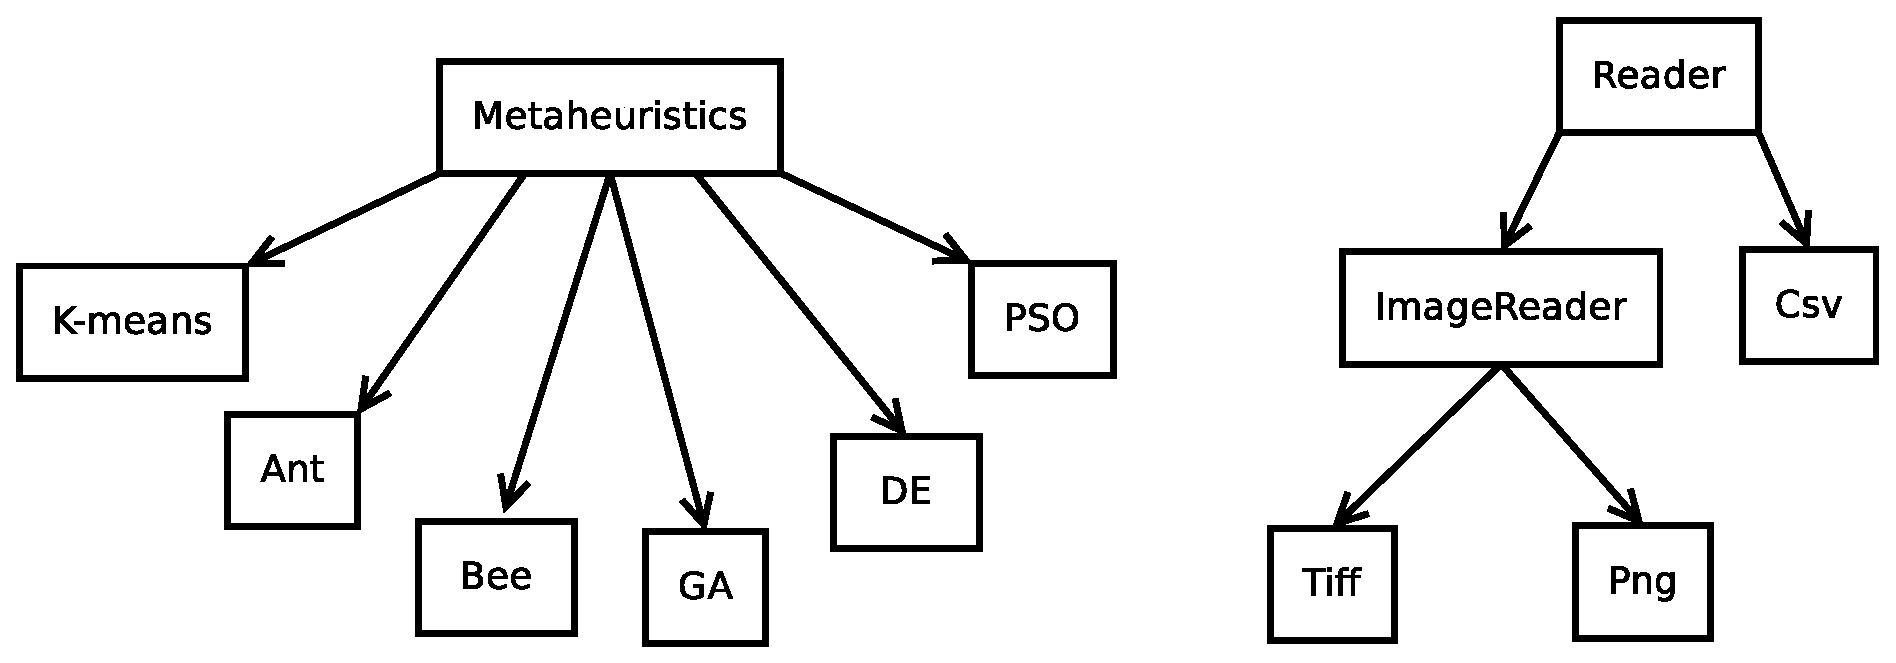
\includegraphics[scale=0.35]{figures/clases.eps}
\caption{Dise\~no de clases}
\label{fig:jclases}
\end{figure}

Donde Metaheuristics es una clase abstracta, que posee las m\'etodos que seran
usados por las diversas metaheur\'isticas hijas. En especial tienen dos 
importantes: initialize y run. El primero se va a encargar de inicializar el algoritmo
para que luego sea ejecutado. Por ejemplo en el gen\'etico inicializa aleatoriamente
las soluciones. Y el run es en s\'i el que va a ejecutar el algoritmo haciendo 
uso de los par\'ametros y variables ya inicilizadas.

Por el otro lado Reader tambi\'en
es una clase abstracta y es la que se encarga de definir lo m\'etodos que van a 
tener sus descendientes a la hora de leer un archivo, que se implement\'o para 
tres tipos: csv, png y tiff.

\section{M'aquina de prueba} \label{sect:testbed}

Todas las pruebas fueron realizadas con el computador cuyas caracter'isticas
aparecen en el cuadro \ref{tb:testbed}. La herramienta {\tt mhs} fue
compilada sobre esa m'aquina, exclusivamente con optimizaci'on gcc de nivel 3,
que es el nivel m\'as alto que posee gcc y aplica todas las mejoras
que este posee.

\begin{table}[htb]
\footnotesize
\begin{center}
\begin{tabular}{|>{\columncolor{lightgray}}c|c|}
\hline
CPU & Intel Core I5 650 \\
\hline
RAM & 6 GB \\
\hline
Distribuci'on & Ubuntu 11.04 x86\_64 bits \\
\hline
Kernel Linux & 2.6.38-8-generic \\
\hline
Versi'on gcc & 4.5.2 \\
\hline
\end{tabular}
\caption{Computador usado para las pruebas}
\label{tb:testbed}
\end{center}
\end{table}

\section{M\'etrica usada}

\section{K-means}

\'Este fue implementado tal cual como se explic\'o en \ref{sect:kmeans}. La
inicializaci\'on es totalmente aleatoria. Y la condici\'on de paradas
va a ser hasta que no se mejores un n\'umero de veces dado.

\section{Bee}

\section{Gen\'etico}

\section{DE}

\section{PSO}

\section{Hormiga}

Los resultados que se quieren evaluar est'an divididos en tres partes: 
Primero, es necesario verificar la calidad de estimaci'on del par'ametro
de Hurst usando los m'etodos implementados, segundo, es importante medir 
el tiempo necesario para cada estimaci'on y, por 'ultimo, es importante
comprobar si se pueden detectar ataques de denegaci'on de servicio mediante la
variaci'on del par'ametro y el uso del mecanismo de ventanas deslizantes.

La descripci'on del computador utilizado para ejecutar las pruebas se 
presenta en la secci'on \ref{sect:testbed}. Los archivos utilizados y los
resultados de la verificaci'on de la estimaci'on del par'ametro de Hurst y del
tiempo necesario para la estimaci'on se presentan en la secci'on
\ref{sect:validacion}. Estos resultandos muestran qu'e tan
preciso es la implementaci'on de los m'etodos y cu'anto tiempo en promedio
necesita la herramienta para estimar el valor del par'ametro de Hurst en una
ventana. 

\section{Validaci'on de los estimados} \label{sect:validacion}

Se ten'ia que probar que las implementaciones de los 3 m'etodos produc'ian
estimaciones razonables del par'ametro de Hurst para saber de antemano que tan
confiable podrian ser la estimaciones cuando se usasen junto con el mecanismo
de ventanas delizantes. Para la validaci'on de los m'etodos implementados se
probaron los mismos con datos producidos por el algoritmo de Paxson
\cite{Paxson95fastapproximation}.

El algoritmo de Paxson permite crear una serie de tiempo pseudo-aleatoria en
el dominio del tiempo de forma r'apida, y permite especificar el par'ametro de
Hurst a ser simulado y el n'umero de datos que debe tener la serie de tiempo
resultante, manteniendo la media en $0$ y la varianza en $1$, con valores
uniformemente distribuidos en el intervalo $[0,2\pi]$. Mediante el algoritmo
se puede simular un proceso estacionario autosimilar con dependencia de largo
alcance \cite{Paxson95fastapproximation}.

La implementaci'on del algoritmo de Paxson utilizada es la que viene en el 
paquete {\tt fArma} de {\tt R}. La validaci'on cont'o con 6 tama~nos diferentes
para la serie de tiempo $X_k$ generada por el algoritmo de Paxson. Estos 
tama~nos fueron $\{1024, 2048, 4096, 8192, 16384, 32768\}$. Por cada tama~no se
generaron 10 series de tiempo $X_k$ para cada uno de los 9 valores del
par'ametro de Hurst que se quer'ia simular. Estos valores fueron
$\{0.55, 0.60, 0.65, 0.70, 0.75, 0.80, 0.85, 0.90, 0.95 \}$. 
\begin{figure}[htb]
\centering
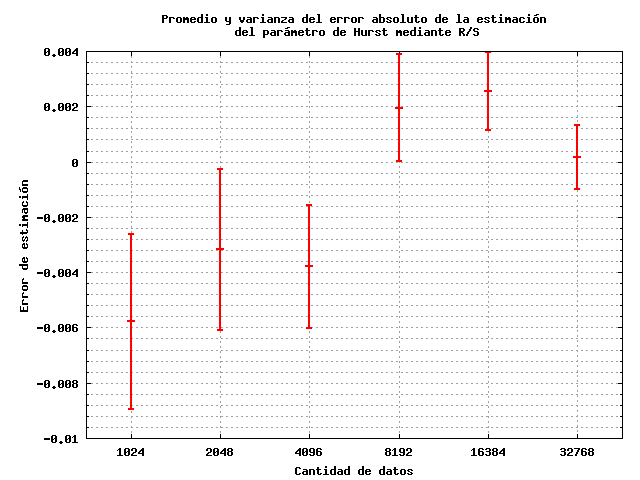
\includegraphics[scale=0.45,type=png,ext=.png,read=.png]{figures/abserror-rs}
\caption{Promedio y varianza del error absoluto de la estimaci'on del par'ametro
de Hurst para el m'etodo estad'istico R/S}
\label{fig:abserrrs}
\end{figure}

\begin{figure}[htb]
\centering
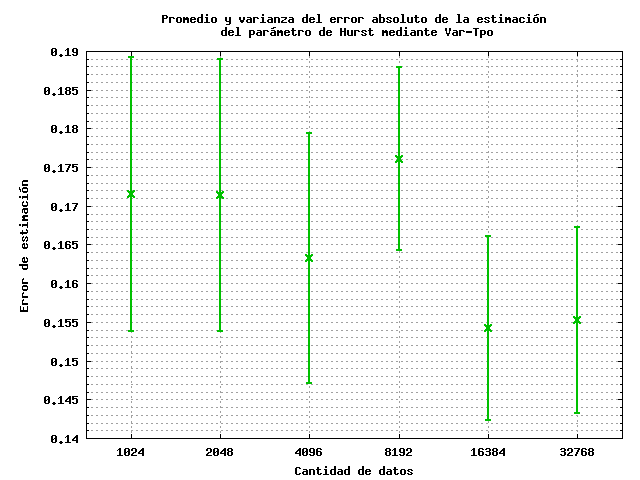
\includegraphics[scale=0.45,type=png,ext=.png,read=.png]{figures/abserror-var}
\caption{Promedio y varianza del error absoluto de la estimaci'on del par'ametro
de Hurst para el m'etodo de gr'aficas de varianza-tiempo}
\label{fig:abserrvar}
\end{figure}

\begin{figure}[htb]
\centering
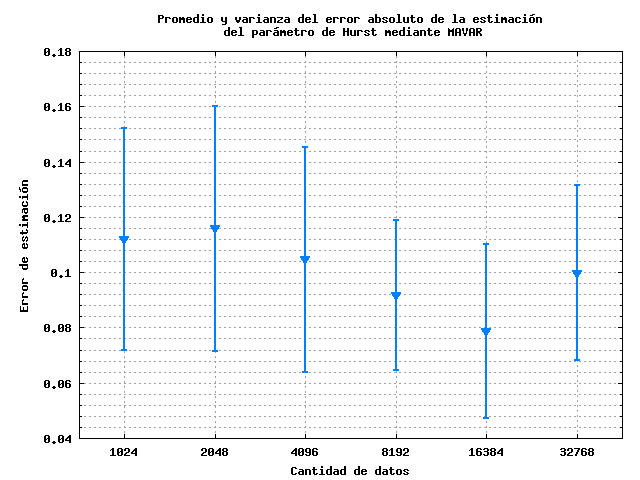
\includegraphics[scale=0.45,type=png,ext=.png,read=.png]{figures/abserror-mavar}
\caption{Promedio y varianza del error absoluto de la estimaci'on del par'ametro
de Hurst para el m'etodo de varianza modificada de Allan}
\label{fig:abserrmavar}
\end{figure}

\clearpage

\begin{figure}[htb]
\centering
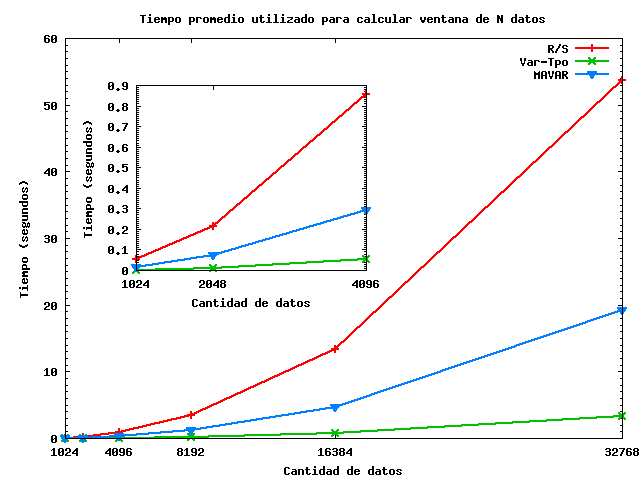
\includegraphics[scale=0.38,type=png,ext=.png,read=.png]{figures/time-n-plot}
\caption{Tiempo promedio utilizado para estimar una ventana de 1024 a 32768
datos para los m'etodos implementados}
\label{fig:tiempoventana}
\end{figure}

Observando las figuras \ref{fig:abserrrs}, \ref{fig:abserrvar} y
\ref{fig:abserrmavar}, lo que se puede evidenciar es que, en general, el
promedio del error absoluto de las estimaciones del par'ametro de Hurst de los
m'etodos mejoran y la varianza disminuye cuando se toman en cuenta un mayor
n'umero de datos para la ventana de estimaci'on. Sin embargo, para los
dos m'etodos que dependen de c'alculos con la varianza el promedio del error 
absoluto de la estimaci'on, incluso con el mayor n'umero de datos es mayor a
$0.1$. El m'etodo del estad'istico R/S es el m'etodo que se comporta mejora 
ya que tiene, en general, un error absoluto muy cerca a $0$ con una varianza
m'inima. 

De acuerdo a \cite{intelligentfuzzy} si queremos analizar los datos en tiempo
real para una red se tendr'ia que hacer una estimaci'on como m'inimo cada
segundo, por lo que una estimaci'on no puede tardar m'as de un segundo en
realizarse. Esto es seriamente limitante ya que cada m'etodo tiene un tiempo de
ejecuci'on muy diferente. Observando la figura \ref{fig:tiempoventana}, con
esta restricci'on la 'unica posibilidad que se tiene es limitar al m'etodo del
estad'istico R/S a $4096$ datos, al m'etodo de gr'aficas varianza-tiempo a
$16834$ datos y al m'etodo de varianza modificada de Allan a $4096$ datos. Dado
que para comparar los m'etodos es importante usar la misma cantidad de datos,
decidimos trabajar con $4096$ datos. El limitar el n'umero de datos va a
afectar la estimaci'on del par'ametro de Hurst directamente como se muestra en
las figuras \ref{fig:abserrrs}, \ref{fig:abserrvar} y \ref{fig:abserrmavar}. 

A pesar de estos problemas, seguimos adelante con el proyecto porque no
queremos una sola estimaci'on puntual y precisa de la traza, sino detectar su
variaci'on, por lo que optamos por un buen balance entre el tiempo de
ejecuci'on y el n'umero de datos a utilizar \cite{intelligentfuzzy}.



% Conclusiones
\chapter{Conclusiones} \label{chap:conclusiones}

    En este capítulo, se presentan los hallazgos y contribuciones de este
proyecto y se dan algunas recomendaciones para futuros trabajos:
\begin{comment}
    Se evaluó el desempeño de los algoritmos \emph{K-means}, \emph{GAH},
\emph{NPSOH}, \emph{WPSOH}, \emph{NDEH}, \emph{SDEH}, \emph{BeeH}, \emph{AntH}.
Estos ocho algoritmos fueron comparados mediante el índice de validez $DB$ y la
cuantificación del error $J_e$ para determinar la calidad de sus soluciones
finales. Además, se comparó el rendimiento de las metaheurísticas \emph{GAH} y
\emph{BeeH} por medio de la cantidad de evaluaciones de su función de \emph{fitness}.
Así que, en función del análisis hecho en el capítulo anterior (ver capítulo \ref{chap:analisis}),
se puede concluir:
\end{comment}

\begin{itemize}
    \item Se llevó a cabo un estudio comparativo entre los algoritmos \emph{K-means},
          \emph{GAH}, \emph{NPSOH}, \emph{WPSOH}, \emph{NDEH}, \emph{SDEH},
          \emph{BeeH} y \emph{AntH} donde \emph{BeeH} y \emph{GAH} resultaron
          ser las mejores metaheurísticas.

    \item Se encontró que \emph{GAH} necesita probabilidades de mutación altas
          ($\geq 0.5$) para que sus soluciones finales sean de calidad.

    \item Se recomienda usar \emph{GAH} cuando no se tenga conocimiento a priori
          del número de clusters.

    \item El índice de validez $DB$ es más eficaz para medir la calidad de una
          partición que la cuantificación de error $J_e$. Esto se debe a que $J_e$
          se ve afectado por la cardinalidad de los clusters.

    \item Las soluciones finales de las metaheurísticas híbridas \emph{NPSOH},
          \emph{WPSOH}, \emph{NDEH}, \emph{SDEH} son similares en calidad. Esto
          puede deberse a que comparten procedimientos.

    \item El \emph{AntH} fue la peor metaheurística implementada. Este comportamiento
          se le atribuye a que no se logró realizar una implementación que
          reprodujera los resultados del artículo \cite{OuBa2007}.

    \item Las metaheurísticas híbridas arrojaron mejores resultados que sus
          contrapartes no híbridas.
          
\end{itemize}

\begin{comment}
\begin{itemize}

	\item El \emph{BeeH} y el \emph{GAH} resultaron ser las mejores metaheurísticas.
    Sin embargo, el \emph{GAH} consiguió soluciones finales con una calidad parecida
    a las del \emph{BeeH} utilizando menos evaluaciones de la función de
    \emph{fitness}.

	\item El \emph{GAH} es la única metaheurística que no requiere la cantidad
    de clusters lo cual es una ventaja cuando no se conoce \emph{a priori}.

	\item Tener una alta probabilidad de mutación ($\geq 0.5$) en el \emph{GAH}
	genera mejores resultados, indicando que el problema de \emph{data clustering}
    necesita grandes modificaciones en los vectores de centroides de sus
    individuos para obtener buenas soluciones.

    \item El índice de validez $DB$ es más eficaz para medir la calidad de una
    partición que la cuantificación del error $J_e$. Esto se debe a que el error
    $J_e$ sugería que la metaheurística \emph{AntH} era la mejor de todas las
    metaheurísticas implementadas. Sin embargo, resultados como los mostrados en
    las figuras \subref{fig:lennaant} y \subref{fig:trivialant}, donde se observa
    mucho ruido, demuestran lo contrario.
    

	\item Las metaheurísticas \emph{NDEH}, \emph{SDEH}, \emph{NPSOH} y \emph{WPSOH}
    comparten un procedimiento para mantener el número de clusters fijo y esto
	podría estar afectando su desempeño, haciendo que sus soluciones sean similares
    entre sí.

	\item El \emph{AntH} fue la peor metaheurística implementada. Este comportamiento
    puede tener su origen en que no se logró hacer una implementación que
    reprodujera los resultados reportados en el artículo base \cite{OuBa2007}.
    En este artículo, no habían suficientes detalles sobre la implementación
    de la memoria de las hormigas y esto pudo haber llevado a una implementación
    ineficiente de la metaheurística \emph{AntH}.
\end{itemize}

\end{comment}

	A partir de los resultados y conclusiones de este proyecto de grado, se pueden
dar las siguientes recomendaciones:

	Primero, es posible que los resultados de las metaheurísticas sean sensibles
a los conjuntos de datos a particionar. Es por esto que todas las metaheurísticas deberían ser probadas
con otros conjuntos de datos, además de \textbf{Lenna} e \textbf{Iris}, de modo
que se corrobore lo dicho en este proyecto de grado.

	Segundo, buscar un nuevo enfoque para la memoria del \emph{AntH}, de modo que
se puedan reproducir los resultados del artículo \cite{OuBa2007}. En este
artículo, no habían suficientes detalles sobre la misma y la implementación
realizada pudo haber afectado el desempeño de esta metaheurística.

	Por último, el procedimiento para mantener los clusters fijos que comparten
las metaheurísticas \emph{NDEH}, \emph{SDEH}, \emph{NPSOH} y \emph{WPSOH} pudo
haber afectado su desempeño. Buscar un nuevo enfoque para este procedimiento,
podría lograr una mejora en los resultados de estas metaheurísticas.


% Crea el glosario 
\printglossaries

% Establece las citas y bibliografia
\bibliographystyle{alpha.bst}
\bibliography{myrefs}

% Crea el apendice
\appendix
% Apendice
\chapter{Informaci'on adicional de {\tt d2Hgr}}

AQU\'I VA EL CONTENIDO DE LOS AP\'ENDICES.
%Puedes quitar esto(es opcional)
\vspace{5 mm}

Esta parte del ap'endice contiene el manual del usuario de la herramienta
implementada, la descripci'on de sus archivos y el c'odigo fuente de algunos
m'odulos de posible inter'es.

\section{Requerimientos de {\it software} y {\it hardware}}
\label{sect:hardsoftrequirements}

El programa resultante deber'ia poder ser utilizado sobre cualquier maquina 
con m'as de 32 MB libres de RAM. Aunque no hay limitaciones para el procesador
a usar, entre m'as nuevo el procesador y mayor n'umero de n'ucleos tenga, m'as
r'apido har'a los calculos la herramienta. En el caso de la memoria, entre 
m'as tenga disponible la herramienta, mayor cantidad de datos podr'a utilizar 
en los c'alculos.

\begin{itemize}
\item Para su compilaci'on, el programa requiere una versi'on actualizada de
gcc, el compilador {\tt C} GNU. Se ha utilizado varias versiones para su
compilaci'on por lo cualquier versi'on mayor a la $4.2$ deber'ia funcionar.
\item La liber'ia {\tt libpcap} es necesaria para darle las funcionalidades de
manipulaci'on de trazas {\tt tcpdump} al programa. A partir de la versi'on
$0.8$ se encuentran todas las funciones que utiliza el programa.
\item La compilaci'on de la herramienta se hace m'as f'acil con {\tt make},
programa GNU. Cualquier versi'on mayor a $3.6$ no deber'ia dar problemas.
\item El programa {\tt gnuplot} es indispensable para poder graficar los
resultados creados por el programa. La versi'on m'as utilizada durante su
desarrollo fue la $4.2$ por lo que es la que se recomienda.
\item La graficaci'on s'olo se puede hacer sobre un sistema operativo bajo el
est'andar POSIX\footnote{"Portable Operating System Interface [for Unix]" son
una familia de est'andares de llamadas al sistema operativo definidos por la
IEEE y especificados formalmente en el IEEE 1003. La gran mayor'ia de las
distribuciones GNU/Linux siguen los est'andares aunque no est'an
oficialmente certificados.} con la herramienta gnuplot instalada. Esto se debe
a una necesidad de la interfaz gnuplot en ANSI C que utiliza un ``pipe'' tipo
POSIX para comunicarse directamente con el programa gnuplot instalado en la
m'aquina. Sin embargo, dentro de las opciones del programa se puede pasar la
informaci'on obtenida en la estimaci'on a archivos de texto para su posterior
an'alisis.
\item La librer'ia pthreads da las funciones necesarias para utilizar hilos
de ejecuci'on en el programa.
\end{itemize}

\section{Ayuda de la l'inea de comando} \label{sect:ayuda}

La herramienta toma como par'ametro principal un archivo {\tt tcpdump} o un CSV
de una serie de tiempo pseudo-aleatoria generada con la herramienta R.
Aparte se puede escoger una velocidad de captura, una ventana, una ventana
deslizante, filtrar paquetes, delimitar corridas, correr con varios hilos de
ejecuci'on, adem'as de estimar el par'ametro de Hurst con los tres m'etodos
mencionados. Se puede tambi'en obtener el cambio del par'ametro de Hurst en el
tiempo o graficar la estimaci'on de una ventana en particular. La ayuda de la
l'inea de comando se muestra abajo:

\begin{alltt}
\label{verb:help}
Usage: ./d2Hgr -[f|g] file -[i|nrlvxmu] [OPTIONS]                               

Estimate and graph Hurst parameter calculations from a file.

   -f file   Specifies a tcpdump dump file.
   -g file   Specifies a CSV file with a simulated network traffic stream.
             This option cannot be used with the time based or tcpdump
             options since the stream is simulated and is static in it's
             definition.
   -i        Prints only the protocol statistic information available from the
             tcpdump file.
   -n        Tells the program if you wish to graph the packets per delta time
             graph. Affected by -p, -o, -d, -c, -b -e, -y flags.
   -r        Tells the program to calculate the Hurst parameter changes over
             time by use of the R/S statistic. Affected by -p, -o, -d, -c, -w,
             -s, -j, -t, -b, -e, -y flags.
   -l num    Tells the program to graph the Pox diagram that creates the Hurst
             data point for a given window number between 0 and Datapoints
             designated by num. Affected by -p, -o, -d, -c, -w, -s, -j, -b,
             -e, -y flags.
   -v        Tells the program to calculate the Hurst parameter changes over
             time by using the Variance-time plot technique. Affected by -p,
             -o, -d, -w, -s, -j, -t, -b, -e, -y flags.
   -x num    Tells the program to graph the Variance-time plot that estimates
             the Hurst parameter for a given window number designated by num.
             Affected by -p, -o, -d, -c, -w, -s, -j, -b, -e, -y flags.
   -m        Tells the program to calculate the Hurst parameter changes over
             time by use of the Modified Allan Variance. Affected by -p, -o,
             -d, -c, -w, -s, -j, -t, -b, -e, -y flags.
   -u num    Tells the program to graph the Modified Allan Variance that
             estimates the Hurst parameter for a given window number designated
             by num. Affected by -p, -o, -d, -c, -w, -s, -j, -t, -b, -e, -y
             flags.

 OPTIONS:
   -p proto  Specifies which protocol to be taken into account when doing
             calculations. Default is all.
             Implemented protocols are:
              ip tcp udp icmp sctp ftp ssh telnet smtp dns dhcp http pop3 ntp
              imap snmp ldap https smtps ldaps imaps pop3s nfs squid
   -o dir    Output directory for results. Default is current directory.
   -d        Tells the program if the results should be placed in text files
             for later use. This option doesn't graph. Useful for using this
             program where gnuplot is not available.
   -y        Tells the program to graph and print the resulting data files.
   -a        Tells the program not to graph or create data files.
   -c sec    Specify a packet capture speed. This makes the program not look
             for one. Example: 0.01 = 0.01 seconds.
   -w sec    Window time size. This makes the program not look for one.
             Example: 60 = 60 seconds.
   -s sec    Slide time size. This makes the program not look for one.
             Example: 1 = 1 seconds.
   -j num    Tells the program to use log base num for all the calculations of
             blocks for the R/S statistic, Variance-time plot and Modified Allan
             Variance. Default is 2.
   -t num    Does Hurst calculation using threads. If 0 is placed, then the
             default number of threads (4) is used.
   -b sec    Tells the program from which second in the time data to begin the
             calculation. Default is 0s.
   -e sec    Tells the program how many seconds after the beginning point to
             include in the calculation. Default is the whole tcpdump time.
   -k num    Average Hurst parameter change with which to try to detect attacks.
   -K num    Standard deviation of Hurst parameter change with which to detect
             attacks.
   -q num    Average Hurst parameter value with which to try to detect attacks.
   -Q num    Standard deviation of Hurst parameter value with which to detect
             attacks.
   -h        Print this help.
\end{alltt}

\section{Archivos del programa}

El programa de C llamado {\tt d2Hgr}, consiste de 18 archivos de c'odigo fuente
que incluye 9 archivos de cabecera. Los archivos contienen la siguiente
informaci'on:

\begin{itemize}
\item{\bf config.h}: Cabecera de funciones para parsear las opciones de linea
de comando.
\item{\bf config.c}: Implementaci'on de las funciones que parsean las opciones
de la linea de comando.
\item{\bf d2Hgr.h}: Archivo que contiene las definiciones de las funciones para
leer los archivos producidos por {\tt tcpdump}.
\item{\bf d2Hgr.c}: Implementaci'on de las funciones para leer la informaci'on
del archivo producido por {\tt tcpdump} y poder obtener la informaci'on
necesaria para su posterior an'alisis.
\item{\bf externvars.h}: Archivo que contiene todas las estructuras especiales
para el uso del programa.
\item{\bf filter.h}: Archivo que contiene la definici'on de las funciones para
construir la expresi'on de filtro de libpcap para usar durante la corrida del
programa.
\item{\bf filter.c}: Archivo que contiene la implementaci'on de todas las
funciones de filter.h.
\item{\bf flows.h}: Cabecera de funciones para contabilizar los flujos de IPv4.
\item{\bf flows.c}: Archivo que contiene la definici'on de las funciones para
contabilizar los flujos de IPv4.
\item{\bf gnuplot\_i.h}: Cabecera para el archivo gnuplot\_i.c que define las
funciones de la interfaz gnuplot para que el programa pueda graficar los
resultados. Esta es una versi'on modificada de la interfaz ANSI C de N.
Devillard para gnuplot.
\item{\bf gnuplot\_i.c}: Implementaci'on de las funciones de N. Devillard para
su interfaz de ANSI C con gnuplot.
\item{\bf graph.h}: Archivo que contiene la definici'on de las funciones para
graficar los resultados.
\item{\bf graph.c}: Archivo que contiene la implementaci'on de las funciones
para graficar los resultados.
\item{\bf hurst.h}: Archivo que contiene las definiciones de los m'etodos para
aproximar el par'ametro de Hurst.
\item{\bf hurst.c}: Archivos que contiene las implementaciones de los m'etodos
para aproximar el par'ametro de Hurst y los m'etodos para extraer la
informaci'on sobre los paquetes una vez leidos por las funciones de d2Hgr.h.
\item{\bf main.c}: El archivo que contiene el main del programa.
\item{\bf detect.h}: El archivo que contiene las definiciones de los m'etodos 
para la detecci'on de ataques de denegaci'on de servicio.
\item{\bf detect.c}: El archivo que contiene las implementaciones de los 
m'etodos para la detecci'on de ataques de denegaci'on de servicio.
\end{itemize}

\section{Creaci'on de $Xtdata$}

\lstinputlisting[caption={Creaci'on de $Xtdata$},label={cod:xtdata}]{code/xtdatacreate.c}




\end{document}
